\documentclass{article}
\usepackage{bigstrut}
\usepackage{adjustbox}
\usepackage{graphicx}^^M
\graphicspath{ {images/} }
\usepackage[T1]{fontenc}
\usepackage{float}

\usepackage[english]{babel}
\usepackage[utf8]{inputenc}
\usepackage{indentfirst}

\addtolength{\oddsidemargin}{-.875in}
\addtolength{\evensidemargin}{-.875in}
\addtolength{\textwidth}{1.75in}
\addtolength{\textheight}{1in}

\begin{document}
\title{Design V: Lab 3}
\begin{titlepage}
    \centering
	{\scshape\LARGE Lab 3: Tensile Testing\par}
	\vspace{1cm}
	{\scshape Aristide Muscariello Jr.: Technician,Recorder \hfill ID\#:10406472 \par}
	{\scshape Marcin Wisniowski: Manager,Technician \hfill ID\#:10417225\par}
	\vfill
	{\scshape Design V, Week 3\par}
	\vspace{.5cm}
	{\scshape Laboratory Performed: February 6th, 2018\\Stevens Institute of Technology\\E-231 Section I Group 2\par}
	\vspace{.5cm}
	{\scshape supervised by\\Mr. Di Wu, Mr. Kai Zong \par}
    \vfill
% Bottom of the page
	{\scshape“I pledge my honor that I have abided by the Stevens Honor System.”\par}
	\vspace{.5cm}
	{\scshape Aristide Muscariello Jr. \hfill Date: 02/11/18\\Marcin Wisniowski \hfill Date: 02/11/18\\}
	\vspace{3cm}
\end{titlepage}

\section{Introduction}
This lab looks to explore the physical properties of materials through a tensile test, a machine operated test that allows to see the maximum stresses that a material can withstand. While undergoing stress, it is common for a material to deform due to the uniaxial tensile forces. Similarly, the modulus of elasticity relates how this deformation occurs for the material under different forces. With a higher modulus of elasticity, the material is able to undergo larger forces with smaller deformations.
	
There are two types of deformations, elastic and plastic. During elastic deformation a material is able to return to its original dimensions after the tensile force is removed. These types of deformations are usually linearly displayed on a tensile test graph. Plastic deformation, however, deforms the material to such an extent that it cannot return to its original dimensions. At a certain point in plastic deformation, there is an ultimate tensile strength that the material can withhold before breaking in two. This is the part of the deformation where the most significant visual changes occur, like necking. 

\subsection{Objective}
Over the course of this lab, the group looks to learn to:
\begin{enumerate}
\item Draw a schematic stress-strain diagram and identify: the elastic region, the plastic region, the yield stress, the ultimate tensile stress, the elongation to failure, and elastic modulus
\item Draw schematic stress-strain diagrams which broadly illustrate the differences in tensile behavior between different materials and materials classes.
\item Describe the role of stress concentrators in the failure of both brittle materials. 
\end{enumerate}

\section{Procedure}
The lab was split into three separate experiments to explore the effects that would occur after putting materials under a load. The group was able to learn the different effects of stress on materials, and also how to control stress conditions in order to create a desired effect. 

\subsection{The Elastic Modulus of Nylon Fishing Line}
The group first explored how a nylon fishing line would deform while being put under stress. A nylon monofilament fishing line was hung from the lab ceiling of a known length. The distance to the ground was measured as a control. Then, a gallon of water was suspended on the bottom of the line and the distance was measured to the ground. The distance was seen to decrease, and an elongation of the nylon fishing line occured due to the addition of the gallon of water. 

\subsection{Tensile Properties of Steel, Aluminum and FRP (Fiber Reinforced Polymer)}
During this experiment, multiple materials were put into a tensile testing machine in order to learn of the properties of each of the materials. The three materials to study are: 

\begin{itemize}
\item 1080 Plain Carbon Steel
\item 6061 Aluminum
\item Fiber Reinforced Polymer
\end{itemize}

Each of these materials has drastically different properties when put under tensile testing. Each was observed for the amount of deformation before snapping and the shape of the fracture that occurred. 

\subsection{Brittle Failure of Glass and the Role of a Stress Concentrator}
The final experiment made the group crack glass under different conditions. First, a control test was used to see how a normal glass microscope slide would crack under normal conditions. Then, a scratch was introduced vertically across the slide to alter the material. Both cracks were observed and recorded with differing effects.

\section{Results}
\subsection{Experiment 1: The Elastic Modulus of Nylon Fishing Line}
The group made multiple initial measurements of the nylon fishing line in order to calculate its Modulus of Elasticity. In order to do this, the group needed to measure the thickness of the nylon line, as well as its length and change of length due to the addition of the gallon of water.

\begin{table}[H]
\begin{center}
\begin{tabular}{c|c|c|c|}
Measurement 1 & Measurement 2 & Measurement 3 & Average \\
\hline
1 mm & .99 mm & 1.1 mm & 1.03 mm\\
\end{tabular}
\caption{Average Thickness of Nylon}
\end{center}
\end{table}

\begin{table}[H]
\begin{center}
\begin{tabular}{c|c|c|c|}
Initial Distance from Ground (in) & Final Distance from Ground (in) & Change in Length (in)\\
\hline
28.75 & 27.5 & 1.25 \\
\end{tabular}
\caption{Length Measurements}
\end{center}
\end{table}

\begin{center}
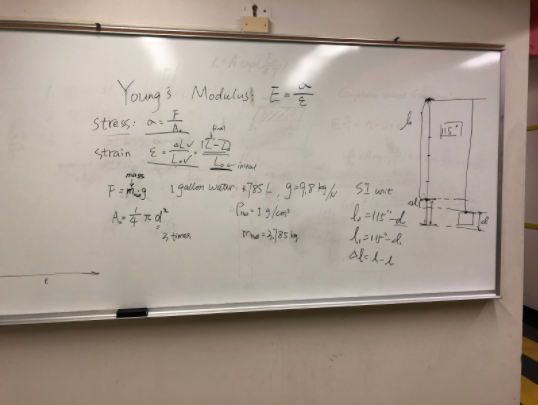
\includegraphics[width=400pt]{NylonEquations.png}
\end{center}

$$Stress: \sigma = \frac{F}{A} \qquad \qquad Strain: \epsilon = \frac{\Delta L}{L_i} \qquad \qquad \Delta L: L_f - L_i$$

$$Stress: \sigma = \frac{F}{A} = \frac{mg}{\pi r^2} = \frac{3.785kg * 9.8 kg/N}{.000515^2 \pi} = 4.45 x 10^7 Pa$$

$$Strain: \epsilon = \frac{\Delta L}{L_i} = \frac{1.25 in}{86.25 in} = .01449275$$

$$Young's Modulus = E = \frac{\sigma}{\epsilon} = 3.07 x 10^9 Pa = 3.07 GPa$$

\begin{table}[H]
\begin{center}
\begin{tabular}{c|c}
Theoretical Young's Modulus & Measured Young's Modulus (Callister)\\
\hline
3.07 GPa & 1.59 GPa\\
\end{tabular}
\caption{Length Measurements}
\end{center}
\end{table}

$$Percent Error = \frac{experimental - theoretical}{theoretical} * 100 = \frac{3.07 GPa - 1.59 GPa}{1.59 GPa} = 93.08$$
\vspace{.5cm}

The first experiment run by the team showed that the fishing line had a Young’s Modulus of 3.07 GPa. The known Young’s Modulus for nylon as found in the textbook is 1.59 GPa. This means the team had an experimental error of 93.08\%. Error in this experiment could have stemmed from how the fishing line had been used by groups before, thus leading to extra fatigue in the line. If the line had been taken beyond its plastic deformation section, the properties would have been changed permanently from what it would have been originally. Another possible source of error could be that the cross section of the fishing line was not uniform throughout. The team had to use an average thickness for the calculations meaning there could be sections of the line that either added to or took away from the final calculated Modulus of Elasticity. However, the expected range for Nylon 66 was found to be between 1.6 GPa and 23 GPa[1] and therefore the error is within expected range.

\subsection{Experiment 2: Tensile Properties of Steel, Aluminum \& FRP}

\begin{center}
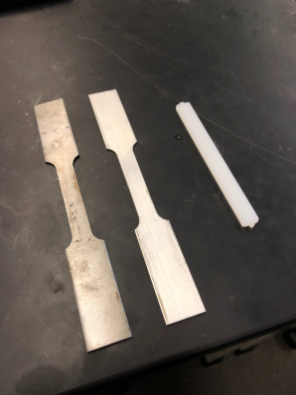
\includegraphics[width=230pt]{TensileTestBefore.png}
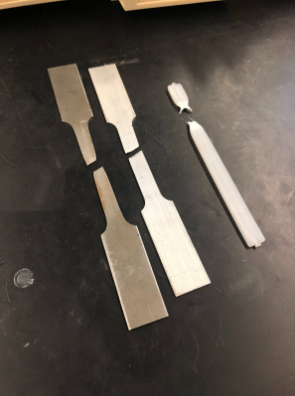
\includegraphics[width=230pt]{TensileTestAfter.png}
\end{center}

\vspace{.5cm}

\renewcommand{\arraystretch}{1.2}
\begin{table}[H]
\begin{center}
\begin{tabular}{c|c|c|c}
Material & Thickness (in) & Width (in) & Initial Length (in)\\
\hline
Steel & 0.0575" & 0.5" & 2.008"\\
\hline
Aluminum & 0.058" & 0.51" & 1.785"\\
\hline
Polymer & 0.1275" & 0.495" & 2.874"\\
\end{tabular}
\caption{Measurements of Materials}
\end{center}
\end{table}

\begin{center}
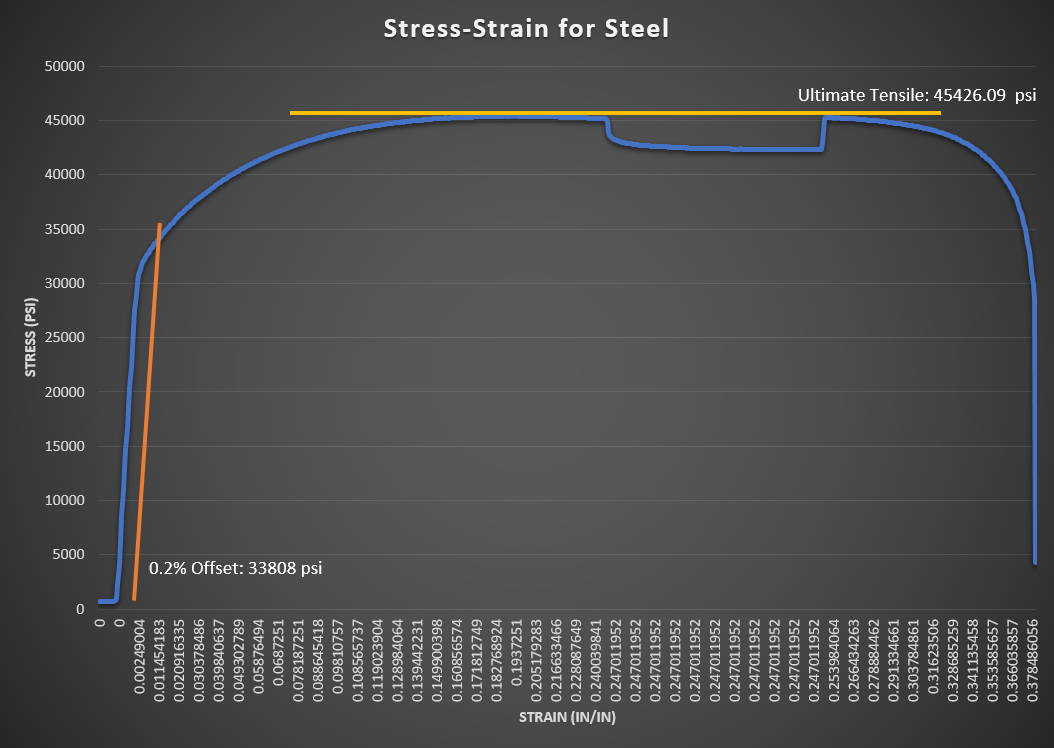
\includegraphics[width=400pt]{SteelGraph.png}
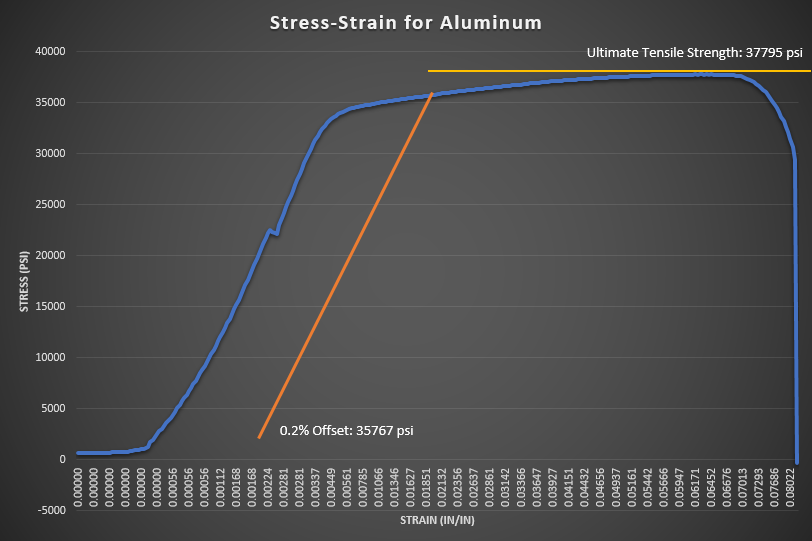
\includegraphics[width=400pt]{AluminumGraph.png}
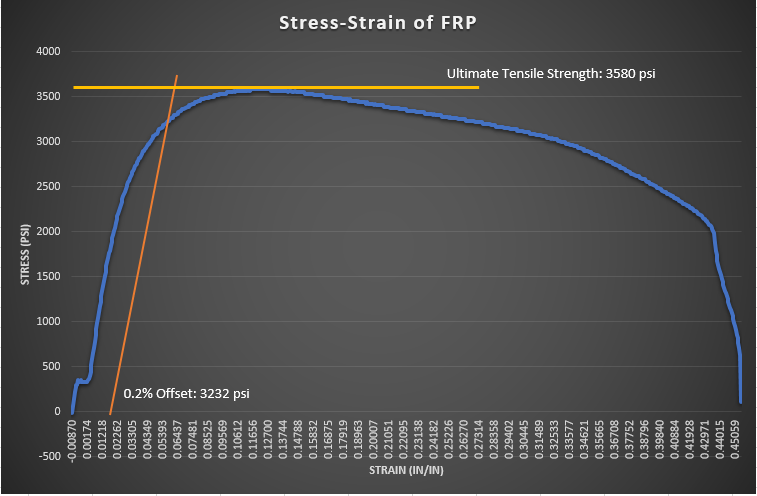
\includegraphics[width=400pt]{PolymerGraph.png}
\end{center}

The graphs generated from this experiment allow the group to find the Young’s Modulus for each material tested. It can be found very easily, as it is simply the slope of the linear line. For the steel and aluminum materials the [2] method was used to gather data, while for the polymer [3] method was used. (See references). 
\paragraph{}
For the Steel tested, the Young’s Modulus is 26,994 ksi. The 0.2\% offset yield is 33,808 psi, the ultimate tensile strength is 45,426 psif and the percent elongation when the material reaches the load at which it fails is 37.998\% elongation. 
\paragraph{}
For Aluminum, the Young’s Modulus is 9,970 ksi. The 0.2\% offset yield is 35,767 psi, the ultimate tensile strength is 37,795 psi and the percent elongation when the material reaches the load at which it fails is 8.190\% elongation. 
\paragraph{}
Finally for the Polymer, the Young’s Modulus is 96.57 ksi. The 0.2\% offset yield is 3232 psi, the ultimate tensile strength is 3580 psi and the percent elongation when the material reaches the load at which it fails is 46.311\% elongation.

\subsection{Experiment 3: Brittle Failure \& Stress Concentration}

\begin{center}
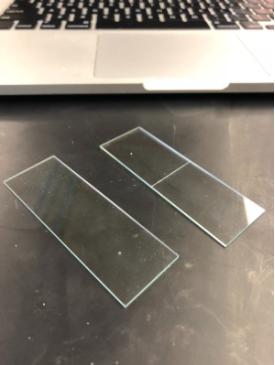
\includegraphics[width=230pt]{GlassBefore.png}
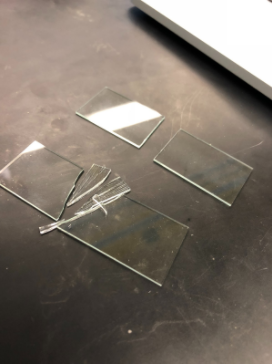
\includegraphics[width=230pt]{GlassAfter.png}
\end{center}

	For the final experiment, the team observed how adding a stress concentrator, in this case a slide with a centered and perpendicular scribe marked in it, can affect how a material will fail. The team broke both the scribed slide and a completely untouched slide to compare how they fail.  The untouched slide broke into a number of pieces that were jagged and unpredictable in size and length. The scribed slide broke almost perfectly along the line scratched into the glass into two clean pieces. A final observation by the team was that in addition to breaking more cleanly than the untouched slide, the scribed slide also required much less force to break.


\section{Conclusion}
In the end, the group learned that different materials behave differently under stress, and that using these properties a better material may be chosen to a given task. The group hypothesized that with higher loads, the nylon would stretch and deform more. Similarly, the group believed that out of 1080 plain carbon steel, 6061 aluminum, and fiber reinforced polymer that the carbon steel will outlast each in both plastic and elastic regions. The group learned that each material has its own positive and negative distinctions when placed under stress. By looking through all of these mechanical properties, a more successful material can be chosen for differing situations. For instance, it can be objectively proven that nylon is better than steel to create a fishing line, because there is a small deformation that is necessary when reeling in a fish, in order to not be pulled overboard. 
 
Finally, the team believes that the way stress is applied alters the way that it breaks. Engineers are able to alter the properties of materials and create their own weak points in order to control where materials would break for them to cause less problems. 

\section{Broader Impacts}
\begin{enumerate}
\item Suppose you repeated the fishing line experiment identically in every detail but instead of using a nylon line you used a fiber of E glass with the identical diameter. What would be the elongation of the E glass fiber? \par

$$E \, glass \, fiber \, elongation: 80 GPa$$
$$E = \frac{Stress}{Strain}$$ 
$$Strain = \sigma = \frac{\Delta L}{L_i}$$
\begin{center}
The Stress will not change if the area diameter will change
\end{center}
$$ 80 GPa = \frac{4.45x10^7 Pa}{\sigma}$$
$$ \sigma = \frac{4.45x10^7 Pa}{80x10^9 Pa}$$
$$ \Delta L = 5.5625x10^{-4} * 86.25 in = 0.048 in$$

\item The FRP composite is a mixture of E-glass and polyethylene. Look up the values of the elastic modulus for these materials. How does the measured elastic modulus of the FRP sample compare? Is it possible to use the elastic modulus of the composite to calculate the fraction of E-glass in the composite? What other method or methods might be used to determine the fraction of fibers in the composite. \par

In order to find the fraction of each material there is, the modulus of elasticity can be put through a weighted distribution of both materials, where each material's elastic modulus is multiplied by the percentage. Another way of finding the fraction of the composite may be to create a chemical reaction that removes on part of the composite and a proportion of masses to figure out the percentage composition. The material we used is approximately 43\% glass and 57\% polyethylene. However, these numbers may be off because there are large ranges of relative Elastic Modulus's for each material. 

\begin{center}
Young's Modulus FRP: 35.5 GPa\par Young's Modulus E-Glass: 80 GPa  \par Young's Modulus Polyethylene (HDE): 0.80 GPa \par

$$35.5 = 80x + .80(1-x)$$
$$35.5 = 79.2x + .80$$ 
$$ x = .43813$$

\end{center}

\end{enumerate}



\section{References}
\paragraph{}
[1]https://www.makeitfrom.com/material-properties/Polyamide-PA-Nylon-6-6-66-Nylon-101
\paragraph{}
[2]Used “Instru-Met Extensometer- Crosshead(pause).msm” Method for Tensile Test of Steel and Aluminum
\paragraph{}
[3]Used E321 = Instru-Met Tensile.msm” Method for Polymer which does not require extensometer


\end{document}